\section{Experimentos e resultados}\label{sec:exp}

\paragraph{Ambiente e protocolo.} Os experimentos rodaram num AMD Ryzen~7
7800X3D (8 núcleos/16 threads, 30~GB), Linux 7.0, Python~3.11.15 e
NumPy~2.4. O limite foi de 30~minutos por execução (heurística mais B\&B);
quem estourou foi registrado como NA, mantendo nós expandidos e podados e o
melhor tour encontrado. A ordem de execução foi:
\begin{enumerate}
  \item as medições sensíveis a tempo (heurísticas, escala e auditoria),
    rodadas \emph{uma de cada vez}, com a máquina sem outra carga;
  \item o B\&B com Held-Karp na TSPLIB, com 4 processos em paralelo;
  \item a escala do B\&B e as instâncias sintéticas, cujas métricas
    principais (nós e custo) não dependem da máquina.
\end{enumerate}
O B\&B com 1-árvore veio de um primeiro lote com 8 processos e não foi
refeito: o código da DFS não mudou, e quase metade dessas 150 execuções
estoura o limite. Nesse lote, árvores idênticas chegaram a levar
2$\times$ mais tempo, então a métrica principal do B\&B é o número de nós.
Todas as 309 execuções do B\&B que terminaram (incluindo as 75 com o GC
desligado) reproduziram o ótimo publicado.

\subsection{Complexidade empírica}\label{sec:complexidade}

Na TSPLIB, $N\in[14,70]$ é estreito demais para distinguir $n^2$ de $n^3$.
Por isso as curvas foram ajustadas em instâncias uniformes no quadrado
$[0,10^4]^2$ (distância EUC\_2D), com $N$ de 25 a 6400 (o blossom só até
1000) e 3 sementes por $N$. A Tabela~\ref{tab:complexidade} traz, para cada
subrotina, duas coisas:
\begin{itemize}
  \item o expoente livre $b$ de $t=aN^b$, ajustado em log-log;
  \item o ajuste do modelo teórico $t=c_0+c_1f(N)$ na escala original, com
    $R^2$ e RMSE, como pede o enunciado.
\end{itemize}

\begin{table}[htb]
\centering
\caption{Ajuste do tempo em função de $N$ (medianas de 3 sementes, $N=25$ a $6400$; blossom até $1000$). $b$: expoente da lei de potência $t=aN^b$ (log-log). Melhor forma: modelo teórico com menor RMSE em escala log. $R^2$/RMSE teoria: ajuste $t=c_0+c_1f(N)$ do modelo teórico em escala linear.}
\label{tab:complexidade}
\small
\begin{adjustbox}{max width=\linewidth}
\begin{tabular}{llcccccc}
\toprule
Algoritmo & Subrotina & Teoria & $b$ (IC 95\%) & $R^2_{\log}$ & Melhor forma & $R^2$ teoria & RMSE (ms) \\
\midrule
Viz. próximo & total & $n^2$ & 1{,}20 $\pm$ 0{,}11 & 0{,}988 & $n\log n$ & 0{,}995 & 0{,}889 \\
Fecho convexo & total & $n^2$ & 1{,}55 $\pm$ 0{,}17 & 0{,}981 & $n\log n$ & 0{,}996 & 42{,}363 \\
TATT & total & $n^2$ & 1{,}20 $\pm$ 0{,}08 & 0{,}993 & $n\log n$ & 0{,}989 & 2{,}113 \\
TATT & MST (Prim) & $n^2$ & 1{,}22 $\pm$ 0{,}08 & 0{,}994 & $n\log n$ & 0{,}990 & 1{,}982 \\
TATT & pré-ordem & $n$ & 0{,}99 $\pm$ 0{,}06 & 0{,}995 & $n$ & 0{,}995 & 0{,}043 \\
Christofides (blossom) & total & $n^3$ & 2{,}81 $\pm$ 0{,}20 & 0{,}996 & $n^3$ & 0{,}997 & 331{,}478 \\
Christofides (blossom) & MST (Prim) & $n^2$ & 1{,}13 $\pm$ 0{,}07 & 0{,}997 & $n\log n$ & 0{,}980 & 0{,}239 \\
Christofides (blossom) & vértices ímpares & $n$ & 0{,}31 $\pm$ 0{,}10 & 0{,}926 & $n$ & 0{,}915 & 0{,}002 \\
Christofides (blossom) & matching: grafo & $n^2$ & 1{,}78 $\pm$ 0{,}27 & 0{,}983 & $n^2$ & 0{,}996 & 0{,}920 \\
Christofides (blossom) & matching: blossom & $n^3$ & 2{,}89 $\pm$ 0{,}15 & 0{,}998 & $n^3$ & 0{,}997 & 333{,}007 \\
Christofides (blossom) & Hierholzer & $n$ & 1{,}01 $\pm$ 0{,}06 & 0{,}997 & $n$ & 0{,}996 & 0{,}018 \\
Christofides (blossom) & atalhos & $n$ & 0{,}82 $\pm$ 0{,}07 & 0{,}994 & $n$ & 0{,}999 & 0{,}000 \\
Christofides (guloso) & total & $n^2\log n$ & 1{,}52 $\pm$ 0{,}20 & 0{,}975 & $n\log n$ & 1{,}000 & 0{,}971 \\
Christofides (guloso) & MST (Prim) & -- & 1{,}23 $\pm$ 0{,}08 & 0{,}993 & $n\log n$ & -- & -- \\
Christofides (guloso) & vértices ímpares & -- & 0{,}32 $\pm$ 0{,}12 & 0{,}828 & $n$ & -- & -- \\
Christofides (guloso) & matching: blossom & $n^2\log n$ & 1{,}82 $\pm$ 0{,}23 & 0{,}977 & $n^2$ & 1{,}000 & 3{,}247 \\
Christofides (guloso) & Hierholzer & -- & 1{,}04 $\pm$ 0{,}03 & 0{,}998 & $n$ & -- & -- \\
Christofides (guloso) & atalhos & -- & 0{,}89 $\pm$ 0{,}06 & 0{,}994 & $n$ & -- & -- \\
\bottomrule
\end{tabular}
\end{adjustbox}
\end{table}


\begin{figure}[htb]
\centering
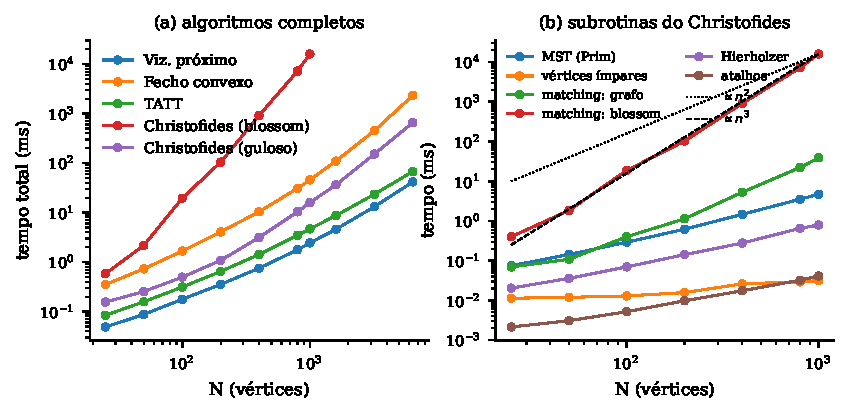
\includegraphics[width=\textwidth]{tempo_vs_n}
\caption{Tempo em função de $N$ (medianas). (a) Algoritmos completos. (b)
Subrotinas do Christofides com retas de referência $\propto n^2$ e
$\propto n^3$.}\label{fig:tempo}
\end{figure}

\paragraph{Onde a teoria aparece.} O blossom segue a teoria com precisão:
$b=2{,}89\pm0{,}15$, contra $O(k^3)$, com $R^2=0{,}997$ para
$c_0+c_1N^3$. Como ele domina, o Christofides inteiro também cresce como
$N^{2{,}81}$. A construção do grafo do matching cresce como $N^{1{,}78}$
($O(k^2)$ arestas), e Hierholzer e pré-ordem são lineares ($b\approx1$).
O matching guloso fica em $N^{1{,}82}$, próximo de $O(k^2\log k)$.

\paragraph{Onde a teoria não aparece.} Prim e vizinho mais próximo são
$O(n^2)$, mas os expoentes medidos foram 1,22 e 1,20. Os dois têm $n$
iterações, cada uma com uma operação NumPy de tamanho $n$. Para $n$ de
milhares, o vetor (até 50~KB) cabe na cache, e a operação vetorizada custa
poucos nanossegundos por elemento, contra microssegundos fixos do
interpretador por iteração. O termo $O(n)$ por iteração só passa a dominar
com $N$ grande: o expoente \emph{local} do Prim, entre $N$ e $2N$, sobe de
0,97 ($N\le100$) para 1,54 (3200 a 6400), e o do vizinho mais próximo de
0,84 para 1,66. A inserção a partir do fecho convexo passa de 2 no fim
(2,37 entre 3200 e 6400), pelos recálculos das inserções invalidadas. Nesse
regime, o modelo teórico ajusta bem na escala linear ($R^2\ge0{,}98$), mas
$n\log n$ descreve melhor a \emph{forma} da curva: até $N\approx10^3$, o
custo prático de um algoritmo $O(n^2)$ vetorizado é dominado pelo número
de iterações do interpretador.

\paragraph{Memória.} A Tabela~\ref{tab:memoria} confirma $O(n^2)$ na
construção do grafo do matching ($b=2{,}01$, 36~MiB em $N=1000$, contra
31~KiB da MST). No matching guloso a memória também é $O(n^2)$ ($b=2{,}03$,
438~MiB em $N=6400$), por causa dos vetores de índices de todos os $k^2/2$
pares. As subrotinas lineares ficam com $b<1$ para $N$ pequeno porque há um
custo fixo de alocação.

\begin{table}[htb]
\centering
\caption{Expoente do pico de memória extra (tracemalloc) em função de $N$.}
\label{tab:memoria}
\small
\begin{adjustbox}{max width=\linewidth}
\begin{tabular}{llcccr}
\toprule
Algoritmo & Subrotina & Teoria & $b$ (IC 95\%) & $R^2_{\log}$ & Pico em $N_{\max}$ (KiB) \\
\midrule
Viz. próximo & total & $n$ & 0{,}75 $\pm$ 0{,}09 & 0{,}977 & 463{,}0 \\
Fecho convexo & total & $n$ & 1{,}32 $\pm$ 0{,}12 & 0{,}989 & 18.257{,}6 \\
TATT & total & $n$ & 0{,}92 $\pm$ 0{,}08 & 0{,}990 & 853{,}3 \\
TATT & MST (Prim) & $n$ & 0{,}55 $\pm$ 0{,}08 & 0{,}968 & 146{,}9 \\
TATT & pré-ordem & -- & 1{,}04 $\pm$ 0{,}03 & 0{,}999 & 802{,}1 \\
Christofides (blossom) & total & $n^2$ & 1{,}87 $\pm$ 0{,}18 & 0{,}993 & 36.358{,}4 \\
Christofides (blossom) & MST (Prim) & $n$ & 0{,}46 $\pm$ 0{,}08 & 0{,}977 & 31{,}5 \\
Christofides (blossom) & vértices ímpares & -- & 0{,}36 $\pm$ 0{,}12 & 0{,}925 & 22{,}3 \\
Christofides (blossom) & matching: grafo & $n^2$ & 2{,}01 $\pm$ 0{,}13 & 0{,}997 & 36.345{,}5 \\
Christofides (blossom) & matching: blossom & $n^2$ & 1{,}07 $\pm$ 0{,}20 & 0{,}975 & 827{,}3 \\
Christofides (blossom) & Hierholzer & -- & 1{,}05 $\pm$ 0{,}04 & 0{,}999 & 386{,}7 \\
Christofides (blossom) & atalhos & -- & 0{,}62 $\pm$ 0{,}16 & 0{,}953 & 9{,}9 \\
Christofides (guloso) & total & $n^2$ & 2{,}00 $\pm$ 0{,}16 & 0{,}990 & 448.597{,}2 \\
Christofides (guloso) & MST (Prim) & -- & 0{,}55 $\pm$ 0{,}08 & 0{,}968 & 146{,}9 \\
Christofides (guloso) & vértices ímpares & -- & 0{,}52 $\pm$ 0{,}13 & 0{,}919 & 112{,}0 \\
Christofides (guloso) & matching: blossom & -- & 2{,}03 $\pm$ 0{,}15 & 0{,}992 & 448.524{,}2 \\
Christofides (guloso) & Hierholzer & -- & 1{,}05 $\pm$ 0{,}02 & 0{,}999 & 2.584{,}7 \\
Christofides (guloso) & atalhos & -- & 0{,}84 $\pm$ 0{,}08 & 0{,}987 & 58{,}4 \\
\bottomrule
\end{tabular}
\end{adjustbox}
\end{table}


\paragraph{Garbage collection.} Toda a escala foi repetida com o GC
desligado (Tabela~\ref{tab:gc}). O Christofides chega a 194 coletas por
execução em $N=1000$, porque o NetworkX cria milhões de objetos Python.
Mesmo assim, a razão entre os tempos com e sem GC ficou entre 0,95 e 1,06
(mediana 1,01), e nenhum expoente mudou mais que 0,02. No B\&B em DFS, a
mediana foi de 0 coletas por execução, e o tempo de CPU com e sem GC
diferiu menos de 2\%. O GC \emph{não} distorce a complexidade aqui.
\begin{itemize}
  \item Os dados grandes vivem em vetores NumPy, que não são rastreados
    pelo GC.
  \item O que cria muitos objetos pequenos é o best-first. Na auditoria,
    desligar o GC aumentou a vazão dele em 2 a 19\%.
  \item As distorções de memória que pesaram foram \emph{cópias}: a cópia
    da matriz inteira no vizinho mais próximo (7,7~MiB em $N=1000$,
    removida) e o grafo completo do NetworkX (49~MiB em $N=500$).
\end{itemize}

\begin{table}[htb]
\centering
\caption{Expoente do tempo total com e sem o coletor de lixo.}
\label{tab:gc}
\small
\begin{adjustbox}{max width=\linewidth}
\begin{tabular}{lcc}
\toprule
Algoritmo & $b$ com GC & $b$ sem GC \\
\midrule
Christofides (blossom) & 2{,}81 & 2{,}80 \\
Christofides (guloso) & 1{,}52 & 1{,}51 \\
Fecho convexo & 1{,}55 & 1{,}54 \\
Viz. próximo & 1{,}20 & 1{,}19 \\
TATT & 1{,}20 & 1{,}19 \\
\bottomrule
\end{tabular}
\end{adjustbox}
\end{table}


\paragraph{Crescimento do B\&B.} Com 10 sementes por $N$ em instâncias
uniformes (Tabela~\ref{tab:bnbescala}, Figura~\ref{fig:bnbescala}), o
número de nós da 1-árvore cresce exponencialmente: cada vértice a mais
multiplica a árvore por 1,54 ($R^2=0{,}986$ no modelo exponencial, contra
0,952 no polinomial). O Held-Karp é tão apertado em pontos uniformes que,
até $N=30$, a DFS desce direto ao ótimo (exatamente $N-2$ nós expandidos).
O crescimento só aparece de $N=35$ em diante e varia muito entre sementes
(fator ajustado de 1,22, $R^2=0{,}88$). O tempo por nó cresce só como
$N^{0{,}65\text{--}0{,}76}$, apesar de ser $O(m^3)$ por nó. É o mesmo
efeito do interpretador visto acima: o Prim em lote tem $m$ iterações
Python, e a aritmética de cada uma é barata. A memória da DFS ficou em
140~KiB com $N=50$.

\begin{table}[htb]
\centering
\caption{Crescimento do B\&B (DFS, filhos por limite, warm-start vizinho mais próximo) em instâncias uniformes. Fator/vértice: $10^{\beta}$ do ajuste $\log_{10}(\text{nós}) = \alpha + \beta N$. $b$ tempo/nó: expoente do tempo de cálculo dos limites por nó expandido; $b$ memória: expoente do pico de memória (tracemalloc) em função de $N$.}
\label{tab:bnbescala}
\small
\begin{adjustbox}{max width=\linewidth}
\begin{tabular}{lcrccccc}
\toprule
Limite & $N$ & Timeouts & Fator/vértice & $R^2$ exp. & $R^2$ polin. & $b$ tempo/nó & $b$ memória \\
\midrule
Held-Karp & 10--50 & 0 & 1{,}21 & 0{,}882 & 0{,}752 & 0{,}65 & 1{,}06 \\
1-árvore & 8--26 & 0 & 1{,}54 & 0{,}986 & 0{,}952 & 0{,}76 & 0{,}88 \\
\bottomrule
\end{tabular}
\end{adjustbox}
\end{table}


\begin{figure}[htb]
\centering
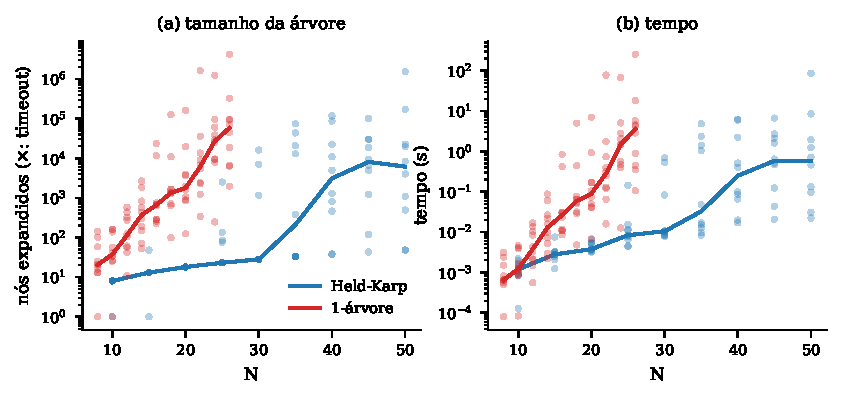
\includegraphics[width=\textwidth]{bnb_escala}
\caption{B\&B (DFS, filhos por LB) em instâncias uniformes, 10 sementes por
$N$; linhas = mediana.}\label{fig:bnbescala}
\end{figure}

\subsection{Impacto do warm-start na árvore de busca}\label{sec:warmstart}

Foram 300 execuções: 15 instâncias $\times$ 5 warm-starts $\times$ 4
configurações. As configurações combinam o limite (Held-Karp ou 1-árvore)
com a ordem dos filhos na DFS (por LB ou por índice). A
Tabela~\ref{tab:warmstart} resume os resultados, e a
Figura~\ref{fig:heatmap} mostra os nós expandidos de cada execução.

\begin{table}[htb]
\centering
\caption{Impacto do warm-start no B\&B (DFS, 15 instâncias, limite de 30 min). Nós exp. (geo): média geométrica dos nós expandidos nas instâncias que todas as estratégias resolveram; razão vs trivial: média geométrica da razão por instância. Posto tempo: posto médio do tempo total (timeout = 1800 s; 1 = mais rápido). Tempo total: soma das 15 execuções.}
\label{tab:warmstart}
\small
\setlength{\tabcolsep}{4pt}
\begin{adjustbox}{max width=\linewidth}
\begin{tabular}{llcrrrrr}
\toprule
Configuração & Warm-start & Resolv. & Gap inicial & Nós exp. (geo) & Razão vs trivial & Posto tempo & Tempo total (s) \\
\midrule
Held-Karp, filhos por LB & Trivial & 15/15 & 152{,}3\% & 193 & 1{,}000 & 2{,}20 & 76 \\
 & Viz. próximo & 15/15 & 24{,}8\% & 244 & 1{,}260 & 2{,}40 & 76 \\
 & Fecho convexo & 15/15 & 2{,}5\% & 129 & 0{,}669 & 2{,}53 & 38 \\
 & TATT & 15/15 & 28{,}5\% & 243 & 1{,}260 & 3{,}07 & 77 \\
 & Christofides & 15/15 & 8{,}1\% & 209 & 1{,}083 & 4{,}80 & 76 \\
\midrule
Held-Karp, filhos por índice & Trivial & 13/15 & 152{,}3\% & 9.236 & 1{,}000 & 4{,}53 & 5.464 \\
 & Viz. próximo & 15/15 & 24{,}8\% & 2.918 & 0{,}316 & 2{,}87 & 1.213 \\
 & Fecho convexo & 15/15 & 2{,}5\% & 224 & 0{,}024 & 1{,}20 & 102 \\
 & TATT & 15/15 & 28{,}5\% & 3.788 & 0{,}410 & 3{,}73 & 2.061 \\
 & Christofides & 15/15 & 8{,}1\% & 1.256 & 0{,}136 & 2{,}67 & 787 \\
\midrule
1-árvore, filhos por LB & Trivial & 9/15 & 152{,}3\% & 384.143 & 1{,}000 & 2{,}80 & 12.886 \\
 & Viz. próximo & 9/15 & 24{,}8\% & 386.606 & 1{,}006 & 3{,}47 & 12.959 \\
 & Fecho convexo & 9/15 & 2{,}5\% & 361.217 & 0{,}940 & 2{,}33 & 12.894 \\
 & TATT & 9/15 & 28{,}5\% & 386.644 & 1{,}007 & 3{,}20 & 12.937 \\
 & Christofides & 9/15 & 8{,}1\% & 385.704 & 1{,}004 & 3{,}20 & 12.942 \\
\midrule
1-árvore, filhos por índice & Trivial & 8/15 & 152{,}3\% & 524.360 & 1{,}000 & 3{,}83 & 14.244 \\
 & Viz. próximo & 8/15 & 24{,}8\% & 429.894 & 0{,}820 & 3{,}30 & 14.225 \\
 & Fecho convexo & 9/15 & 2{,}5\% & 261.998 & 0{,}500 & 2{,}20 & 13.427 \\
 & TATT & 8/15 & 28{,}5\% & 457.197 & 0{,}872 & 3{,}03 & 14.190 \\
 & Christofides & 8/15 & 8{,}1\% & 344.515 & 0{,}657 & 2{,}63 & 14.063 \\
\bottomrule
\end{tabular}
\end{adjustbox}
\end{table}


\begin{figure}[htb]
\centering
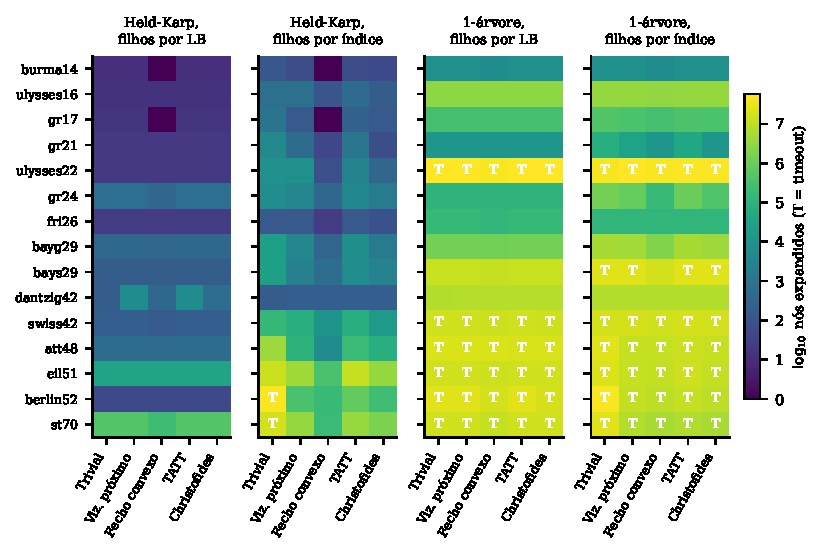
\includegraphics[width=\textwidth]{warmstart_heatmap}
\caption{Nós expandidos ($\log_{10}$) por instância, estratégia e
configuração. T: estourou 30 minutos.}\label{fig:heatmap}
\end{figure}

\paragraph{Quando o warm-start importa.} Com filhos visitados por índice, a
DFS não tem guia: no começo, a única fonte de poda é a incumbente. Nesse
regime a qualidade do limite superior inicial decide o tamanho da árvore.
Com Held-Karp e filhos por índice:
\begin{itemize}
  \item a solução trivial (gap inicial médio de 152\%) deixou berlin52 e
    st70 sem terminar em 30~minutos;
  \item todas as heurísticas resolveram as 15 instâncias;
  \item a inserção a partir do fecho convexo (gap médio de 2,5\%) expandiu
    em média 41$\times$ menos nós que a trivial (razão geométrica 0,024), o
    Christofides 7$\times$ menos (0,136), o vizinho mais próximo 3$\times$
    e o TATT 2,4$\times$.
\end{itemize}
O tempo total das 15 execuções caiu de 5464~s (trivial) para 102~s (fecho).
Dentro de cada instância, o número de nós acompanha o gap inicial
(correlação de Spearman média de 0,97). Os perfis por profundidade
(Figura~\ref{fig:profundidade}) mostram o mecanismo: com um UB bom, a poda
começa nos níveis rasos, e a árvore nem chega a abrir os ramos ruins.

\paragraph{Quando quase não importa.} Com filhos ordenados por LB, a
primeira descida da DFS já se comporta como uma heurística gulosa guiada
pelo limite. Com Held-Karp ela encontra um tour ótimo ou quase ótimo em
milissegundos, e o UB inicial deixa de ser a fonte principal de poda.
\begin{itemize}
  \item As 15 instâncias foram resolvidas com qualquer warm-start, e as
    razões de nós ficaram entre 0,67 (fecho) e 1,26.
  \item Um UB inicial melhor pode até \emph{aumentar} a árvore. No
    dantzig42, a solução trivial é ótima (699) e levou a 190 nós; o vizinho
    mais próximo levou a 6078. A diferença está no desempate: com outra
    incumbente, a primeira descida segue outro ramo de mesmo LB.
\end{itemize}
Com a 1-árvore, os dois regimes se confundem. O limite é tão fraco (gap de
10 a 31\% na raiz) que as árvores têm milhões de nós de qualquer forma. As
razões ficam entre 0,94 e 1,01 com filhos por LB, e entre 0,50 e 0,87 com
filhos por índice. O teste de Friedman (Tabela~\ref{tab:friedman}) não
rejeita a igualdade do tempo entre as estratégias com 1-árvore e filhos por
LB ($p=0{,}10$), e rejeita com folga nas configurações em que o UB
importa.

\begin{figure}[htb]
\centering
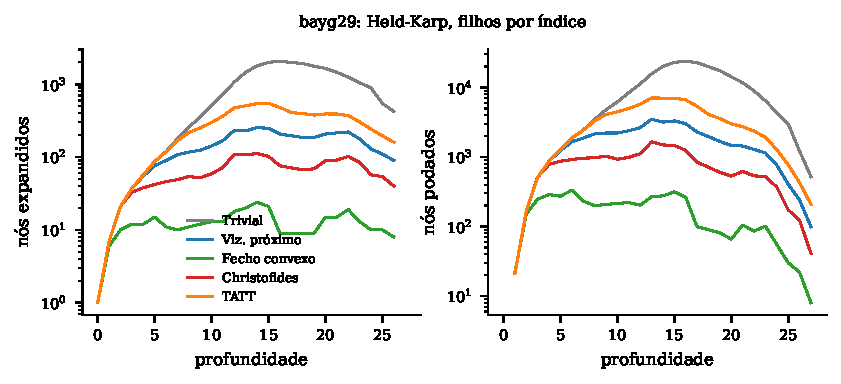
\includegraphics[width=\textwidth]{warmstart_profundidade_bayg29}
\caption{Nós expandidos e podados por profundidade, bayg29 (Held-Karp,
filhos por índice).}\label{fig:profundidade}
\end{figure}

\begin{table}[htb]
\centering
\caption{Teste de Friedman (4 graus de liberdade) para a hipótese de que as cinco estratégias de warm-start têm o mesmo desempenho.}
\label{tab:friedman}
\small
\begin{adjustbox}{max width=\linewidth}
\begin{tabular}{lcccc}
\toprule
Configuração & $\chi^2_F$ tempo & $p$ tempo & $\chi^2_F$ nós & $p$ nós \\
\midrule
Held-Karp, filhos por LB & 26{,}8 & 2{,}2e-05 & 25{,}8 & 3{,}5e-05 \\
Held-Karp, filhos por índice & 37{,}5 & 1{,}4e-07 & 38{,}3 & 9{,}6e-08 \\
1-árvore, filhos por LB & 7{,}8 & 9{,}8e-02 & 26{,}0 & 3{,}1e-05 \\
1-árvore, filhos por índice & 16{,}5 & 2{,}4e-03 & 24{,}1 & 7{,}6e-05 \\
\bottomrule
\end{tabular}
\end{adjustbox}
\end{table}


\paragraph{O tempo da heurística compensa?} Sim, sempre que o UB importa.
As heurísticas levaram de 0,08~ms (vizinho mais próximo) a 1,7~ms
(Christofides, mediana), e no máximo 8,8~ms. Com Held-Karp e filhos por
índice, a economia de tempo superou o custo da heurística em 13 a 14 das 15
instâncias, num total de 3400 a 5360~s economizados contra menos de 0,04~s
gastos. Com filhos por LB, o B\&B inteiro leva dezenas de milissegundos nas
instâncias pequenas. Aí os 1,7~ms do Christofides chegam a pesar mais que a
busca, e ele ficou com o pior posto médio de tempo (4,8). O vizinho mais
próximo é o que melhor equilibra custo e qualidade quando não se sabe a
ordem dos filhos; o fecho convexo é o melhor em qualidade a um custo ainda
desprezível (0,5~ms).

\paragraph{Ponto de colapso.} A Tabela~\ref{tab:colapso} mostra onde o
B\&B exato deixa de terminar em 30~minutos. Com Held-Karp e filhos por LB,
todas as 15 instâncias foram resolvidas, até o st70, em no máximo 72~s. Com
filhos por índice, o primeiro timeout foi em $N=52$ (berlin52, só com a
trivial). Com a 1-árvore, o colapso começa em $N=22$ (ulysses22), e
nenhuma instância com $N\ge48$ terminou. Entre 22 e 42, ele depende da
instância: dantzig42 terminou, swiss42 não. Mesmo nesses casos, os
aproximativos rodam em milissegundos (Seção~\ref{sec:complexidade}).

\begin{table}[htb]
\centering
\caption{Ponto de colapso do B\&B exato na TSPLIB (30 min).}
\label{tab:colapso}
\small
\begin{adjustbox}{max width=\linewidth}
\begin{tabular}{lcccc}
\toprule
Configuração & Resolvidas (alguma) & Resolvidas (todas) & Maior $N$ resolvido & Menor $N$ com timeout \\
\midrule
Held-Karp, filhos por LB & 15/15 & 15/15 & 70 & -- \\
Held-Karp, filhos por índice & 15/15 & 13/15 & 70 & 52 \\
1-árvore, filhos por LB & 9/15 & 9/15 & 42 & 22 \\
1-árvore, filhos por índice & 9/15 & 8/15 & 42 & 22 \\
\bottomrule
\end{tabular}
\end{adjustbox}
\end{table}

\begin{table}[htb]
\centering
\caption{Profiling do B\&B: mediana, nas 75 execuções de cada configuração, da fração do tempo total em cada subrotina, e tempo de cálculo dos limites por nó expandido. O restante é a própria busca (recursão, ordenação).}
\label{tab:perfil}
\small
\begin{adjustbox}{max width=\linewidth}
\begin{tabular}{lrrrr}
\toprule
Configuração & Heurística & Limite na raiz & Limites dos filhos & $\mu$s por nó \\
\midrule
Held-Karp, filhos por LB & 0{,}75\% & 50{,}9\% & 44{,}8\% & 59 \\
Held-Karp, filhos por índice & 0{,}08\% & 6{,}7\% & 83{,}0\% & 48 \\
1-árvore, filhos por LB & 0{,}00\% & 0{,}0\% & 94{,}4\% & 67 \\
1-árvore, filhos por índice & 0{,}00\% & 0{,}0\% & 90{,}7\% & 68 \\
\bottomrule
\end{tabular}
\end{adjustbox}
\end{table}


\subsection{Sensibilidade às características das instâncias}\label{sec:sens}

Quinze instâncias são poucas para um modelo com 13 features. Geramos então
168 instâncias sintéticas \emph{adversariais}, com $N\in\{20,30,40,50\}$ e 6
sementes, em sete famílias. Cada família estressa uma feature pedida:
\begin{itemize}
  \item \emph{uniforme}: a referência;
  \item \emph{aglomerados}: silhueta alta e Clark-Evans $<1$;
  \item \emph{grade}: Clark-Evans $>1$ e muitos empates no vizinho mais
    próximo;
  \item \emph{anel}: quase todos os pontos no fecho;
  \item \emph{faixa}: razão de aspecto entre 0,05 e 0,2;
  \item \emph{núcleo denso e pontos dispersos}: alto CV da distância ao
    vizinho mais próximo;
  \item \emph{raios}: hubs na MST.
\end{itemize}
O ótimo exato de cada uma veio do B\&B com Held-Karp, com limite de 15~min;
159 das 168 foram resolvidas, e o gap de cada heurística é exato. O
índice de Clark-Evans~\cite{clarkevans1954} usa a correção de borda de
Donnelly~\cite{donnelly1978}. Sem ela, com $N$ pequeno, todas as 15
instâncias da TSPLIB davam $>1$, até as claramente agrupadas. A base final
tem 174 instâncias, e os modelos são avaliados por validação cruzada
(5 partes, 10 repetições).

\begin{table}[htb]
\centering
\caption{Mediana do gap (\%) por família de instância. A última coluna é o gap do limite de 1-árvore na raiz do B\&B.}
\label{tab:familias}
\small
\begin{adjustbox}{max width=\linewidth}
\begin{tabular}{lrrrrrrr}
\toprule
Família & Inst. & Viz. próximo & Fecho convexo & TATT & Christofides & Christ. guloso & gap raiz 1-árvore \\
\midrule
uniforme & 24 & 20{,}1 & 3{,}3 & 35{,}4 & 10{,}4 & 13{,}6 & 11{,}9 \\
aglomerados & 18 & 16{,}4 & 1{,}2 & 19{,}2 & 6{,}8 & 11{,}9 & 27{,}1 \\
grade & 24 & 27{,}2 & 5{,}3 & 32{,}8 & 13{,}2 & 20{,}5 & 5{,}4 \\
anel & 24 & 0{,}0 & 0{,}0 & 23{,}0 & 0{,}0 & 0{,}0 & 5{,}8 \\
faixa & 22 & 18{,}7 & 0{,}1 & 15{,}6 & 9{,}6 & 18{,}9 & 25{,}5 \\
núcleo+dispersos & 23 & 16{,}5 & 2{,}9 & 17{,}0 & 7{,}3 & 13{,}2 & 28{,}2 \\
raios & 24 & 18{,}2 & 2{,}5 & 25{,}2 & 8{,}8 & 13{,}5 & 26{,}8 \\
TSPLIB & 15 & 22{,}1 & 2{,}2 & 31{,}0 & 7{,}5 & 17{,}2 & 15{,}0 \\
\bottomrule
\end{tabular}
\end{adjustbox}
\end{table}


\paragraph{Instâncias adversariais.} Cada família estressa as heurísticas
de um jeito (Tabela~\ref{tab:familias}, Figura~\ref{fig:familias}):
\begin{itemize}
  \item \emph{Grade} é a pior para quase todas: o vizinho mais próximo
    chega a 27\% de gap, e o Christofides a 13\%. Com distâncias quase
    iguais, as escolhas locais empatam, e os desempates errados se acumulam.
  \item \emph{Anel} é trivial para todas as heurísticas, menos o TATT (23\%
    de gap): a MST de pontos num círculo é um caminho, e a pré-ordem a
    percorre bem, mas a aresta de volta atravessa o anel.
  \item Para o limite de 1-árvore, as piores são as estruturadas:
    aglomerados, núcleo com dispersos, faixa e raios, todas com 25 a 28\%
    de gap na raiz, contra 12\% na uniforme e 5\% na grade. A MST liga os
    grupos com poucas arestas longas e tem muitas folhas, então fica longe
    de um caminho hamiltoniano.
\end{itemize}
O Held-Karp corrige os graus com as penalidades $\pi$ e fechou essa
diferença: mediana de 0 a 0,2\% em todas as famílias.

\begin{figure}[htb]
\centering
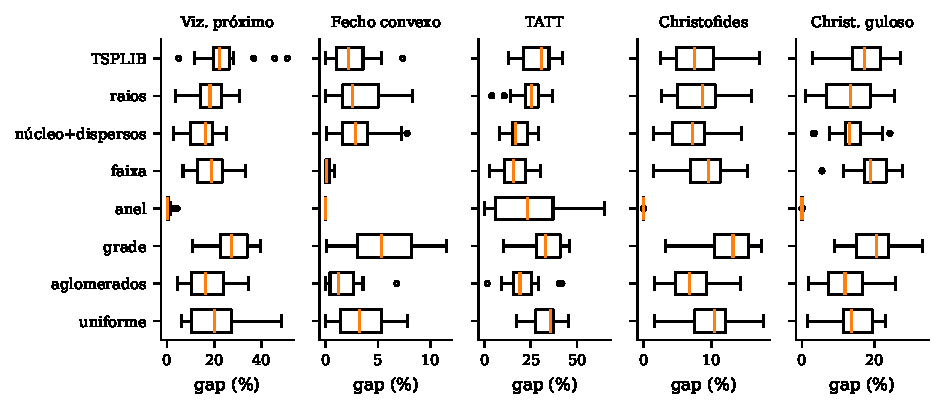
\includegraphics[width=\textwidth]{sensibilidade_familias}
\caption{Gap por família (instâncias sintéticas com ótimo exato e TSPLIB).}\label{fig:familias}
\end{figure}

\begin{figure}[htb]
\centering
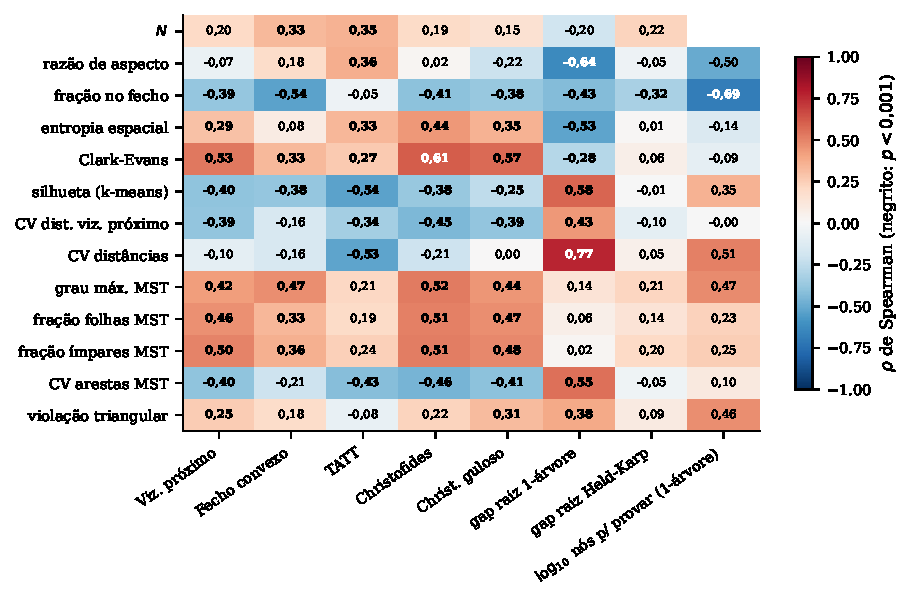
\includegraphics[width=0.95\textwidth]{sensibilidade_spearman}
\caption{Correlação de Spearman entre features e gaps nas 174 instâncias.}\label{fig:spearman}
\end{figure}

\paragraph{Peso das features.} A Figura~\ref{fig:spearman} mostra as
correlações. Para os modelos, três features com VIF $>10$ foram removidas
(fração de folhas da MST, CV das arestas da MST e CV das distâncias).
Sobraram 10 features padronizadas para a regressão múltipla
(Tabela~\ref{tab:coeficientes}), a árvore de decisão de profundidade 3
(Figura~\ref{fig:arvore}) e a floresta aleatória~\cite{breiman2001}.
\begin{itemize}
  \item \emph{Fração de pontos no fecho convexo.} É a feature mais forte e
    consistente: um desvio padrão a mais reduz o gap do Christofides em
    2,2 pontos percentuais e o do vizinho mais próximo em 2,5. Ela também é
    a primeira divisão das árvores. Com mais de 47\% dos pontos no fecho,
    o gap médio do Christofides fica abaixo de 0,5\%.
  \item \emph{Clark-Evans e entropia espacial} pioram o Christofides
    ($+2{,}1$ cada, $p<0{,}001$). Pontos regulares e espalhados são o caso
    difícil, como na família grade.
  \item \emph{Fração de vértices ímpares na MST} pesa no vizinho mais
    próximo e no TATT ($+3{,}5$ e $+4{,}6$). Ela é proporcional ao tamanho
    do matching e mede quanto a MST se ramifica. O grau máximo da MST
    (hubs) tem efeito pequeno: $+0{,}7$ no Christofides, $p=0{,}02$.
  \item \emph{O gap do limite de 1-árvore na raiz} é o mais previsível
    ($R^2_{CV}=0{,}83$). Ele cai com a fração no fecho ($-6{,}9$), com $N$
    e com Clark-Evans, ou seja, é maior em instâncias agrupadas.
\end{itemize}
Os gaps das heurísticas são explicados só em parte: o $R^2_{CV}$ fica entre
0,30 (TATT) e 0,58 (Christofides). O resto depende de detalhes
combinatórios, como empates e a ordem dos vértices, que as features globais
não capturam. A árvore de decisão sozinha generaliza pior que a regressão
(Tabela~\ref{tab:modelos}), mas suas regras são legíveis e coincidem com
os coeficientes.

\begin{table}[htb]
\centering
\caption{Coeficientes padronizados da regressão múltipla (variação do gap, em pontos percentuais, por desvio padrão da feature). $^{*}p<0{,}05$, $^{**}p<0{,}01$, $^{***}p<0{,}001$.}
\label{tab:coeficientes}
\small
\begin{adjustbox}{max width=\linewidth}
\begin{tabular}{lrrrrrr}
\toprule
Feature & Viz. próximo & Fecho convexo & TATT & Christofides & Christ. guloso & gap raiz 1-árvore \\
\midrule
$N$ & 1{,}07 & 0{,}39$^{*}$ & 4{,}09$^{***}$ & 0{,}14 & 0{,}82 & -3{,}91$^{***}$ \\
razão de aspecto & -1{,}70 & 0{,}71$^{**}$ & 2{,}75$^{**}$ & 1{,}01$^{**}$ & -1{,}23$^{*}$ & -3{,}53$^{***}$ \\
fração no fecho & -2{,}45$^{*}$ & -0{,}74$^{**}$ & 2{,}30 & -2{,}20$^{***}$ & -2{,}90$^{***}$ & -6{,}91$^{***}$ \\
entropia espacial & 0{,}02 & -0{,}55 & 1{,}19 & 2{,}15$^{***}$ & 1{,}57 & -2{,}00$^{**}$ \\
Clark-Evans & 0{,}90 & 1{,}03$^{**}$ & -2{,}24 & 2{,}14$^{***}$ & 2{,}93$^{**}$ & -3{,}63$^{***}$ \\
silhueta (k-means) & -3{,}14$^{*}$ & -0{,}50 & -3{,}65$^{*}$ & 1{,}47$^{**}$ & 0{,}99 & 0{,}62 \\
CV dist. viz. próximo & 0{,}10 & 0{,}08 & -0{,}34 & 0{,}63 & 0{,}39 & -0{,}04 \\
grau máx. MST & 0{,}52 & 0{,}39 & 0{,}68 & 0{,}70$^{*}$ & 0{,}35 & 0{,}09 \\
fração ímpares MST & 3{,}50$^{**}$ & -0{,}33 & 4{,}58$^{***}$ & 0{,}76 & 1{,}63$^{*}$ & -1{,}16$^{*}$ \\
violação triangular & -0{,}58 & -0{,}05 & -0{,}00 & -0{,}05 & 0{,}70 & -0{,}20 \\
\bottomrule
\end{tabular}
\end{adjustbox}
\end{table}

\begin{table}[htb]
\centering
\caption{Poder preditivo das features (validação cruzada 5-fold repetida). Linear: regressão múltipla padronizada; árvore: profundidade 3; floresta: 300 árvores.}
\label{tab:modelos}
\small
\begin{adjustbox}{max width=\linewidth}
\begin{tabular}{lrcccc}
\toprule
Alvo & Inst. & $R^2$ treino (lin.) & $R^2_{CV}$ linear & $R^2_{CV}$ árvore & $R^2_{CV}$ floresta \\
\midrule
Viz. próximo & 174 & 0{,}51 & 0{,}40 & 0{,}31 & 0{,}40 \\
Fecho convexo & 174 & 0{,}49 & 0{,}39 & 0{,}22 & 0{,}37 \\
TATT & 174 & 0{,}41 & 0{,}30 & 0{,}16 & 0{,}20 \\
Christofides & 174 & 0{,}65 & 0{,}58 & 0{,}38 & 0{,}56 \\
Christ. guloso & 174 & 0{,}60 & 0{,}50 & 0{,}38 & 0{,}48 \\
gap raiz 1-árvore & 174 & 0{,}86 & 0{,}83 & 0{,}47 & 0{,}72 \\
$\log_{10}$ nós p/ provar (1-árvore) & 33 & 0{,}83 & 0{,}19 & -0{,}73 & 0{,}33 \\
\bottomrule
\end{tabular}
\end{adjustbox}
\end{table}


\begin{figure}[htb]
\centering
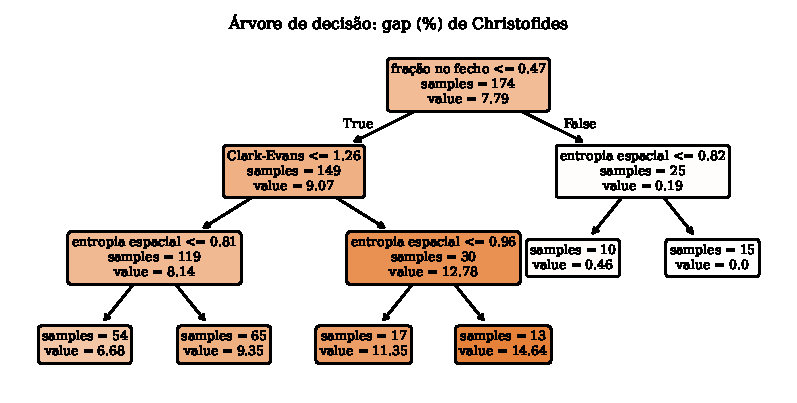
\includegraphics[width=\textwidth]{arvore_christofides}
\caption{Árvore de decisão (profundidade 3) para o gap do Christofides;
valor = gap médio (\%) da folha.}\label{fig:arvore}
\end{figure}

\paragraph{Por que a 1-árvore falhou no ulysses22.} O ulysses22 é o menor
$N$ em que o B\&B com 1-árvore estourou 30~minutos. Ele tem o maior CV da
distância ao vizinho mais próximo da TSPLIB (1,63; a mediana é 0,60) e um
dos maiores gaps de 1-árvore na raiz (30,6\%, igual ao do ulysses16 e
contra 9,6 a 19,7\% das instâncias com $N\ge24$). Os pontos são ilhas e
cidades do Mediterrâneo: grupos densos separados por grandes distâncias.
Nessa geometria, a MST junta cada grupo com arestas curtas e liga os grupos
com poucas arestas longas. Muitos vértices ficam com grau diferente de 2, e
a árvore está longe de um tour. O limite fica muito abaixo do ótimo em
todos os níveis, e quase nada é podado: foram de 44 a 57 milhões de nós
expandidos em 30~minutos, conforme a estratégia. O Held-Karp penaliza exatamente esses graus, deixou o gap na
raiz em 0,00\% e resolveu a instância com 20 nós.
